Using logic grid puzzles as a use-case, we will validate the feasibility of finding a sequence of small explanations.

As data we use puzzles from Puzzle Baron’s Logic Puzzles Volume 3~\cite{logigrammen}. The first 10 puzzles were used to construct the grammar. Using this grammar, and a semi-automatically problem-specific lexicon, we are able to parse and solve all puzzles in the booklet, including those not used to construct the grammar. Our experiments below are on test puzzles not used to construct the grammar; we also report results on the \textit{pasta} puzzle, which was emailed to us by a person that did not manage to solve it himself.\tias{do we know the source of the original puzzle?}

As constraint solving engine, we use IDP~\cite{IDP}. It is a knowledge representation and reasoning system that supports multiple queries on a first order logic theory. We will use the 'optimalpropagate()' query, which efficiently finds the maximally consistent (partial) interpretation of a theory, which in our case is a full interpretation, e.g. the solution to the logic grid puzzle. We also use the 'findMUS()'\tias{Bart, how is it really name?} query that searches for a subset-minimal unsatisfiable core.

The algorithm itself is written in embedded LUA, which is provided as en imperative environment inside the otherwise declarative IDP system. The code was not optimized for efficiency and can at this point not be used in an interactive setting, as it takes between 15 minutes to a few hours to fully explain a logic grid puzzle. Experiments were run on an Intel(R) Xeon(R) CPU E3-1225 with 4 cores and 32 Gb memory, running linux 4.15.0 and IDP version 3.7.1.

\paragraph{1. Sequence composition}
We first look at the properties of the puzzles and the composition of the resulting sequence explanations. The results are shown in Table~\ref{table:composition}. The bottom puzzle is the pasta puzzle. $|type|$ is the number of types of entities (e.g. person, sauce) while $|dom|$ is the number of entities of each type. $|grid|$ is the number of cells in the grid, e.g. the number of literals in the maximal consequence interpretation $I_n=max(I_0,\allconstraints)$.

Coincidentally, the puzzles all have 4 types with a domain of size 5, and hence 150 cells. We can see that the number of inference steps is around 120 for all but the pasta puzzle. When looking at the proportion of the inference steps that use bijections (only), transitivity (only) or a clue, we can see that around 50\% the explanations typically use a transitivity constraint, around 25\% typically a trivial bijectivity constraint (e.g. completing a row or column in one relation), and less then $1/5$th of the explanations actually need to use a clue.
In the table, \#m-i and \#m-c refer to the use of multiple implicit constraints and multiple clues respectively. We can see that it is never necessary to combine multiple constraints in one inference step. Also, notably, the puzzles from the booklet never require combining implicit constraints, while the anecdotically hard pasta puzzle is the only one that does, e.g. it can not be solved by focussing on the clues but one must combine facts and knowledge in the table alone to crack it.

\begin{table}
	\centering
	\resizebox{\columnwidth}{!}{%
\begin{tabular}{c|ccc|c|cccccc} 
	\textbf{puzzle} & \textbf{$|$type$|$} & \textbf{$|$dom$|$} & \textbf{$|$grid$|$} & \textbf{steps} & \textbf{\% Bij.} & \textbf{\% Trans.} & \textbf{\% 1 Clue} & \textbf{\% m-i} & \textbf{\% m-c} \\ 
				\hline 
				%p5.output.json
				1 & 4 & 5 & 150 & 113 & 31.0 & 31.0 & 18.6 & 0.0 & 0\\ 
				%p16.output.json
				2 & 4 & 5 & 150 & 122 & 21.3 & 21.3 & 18.9 & 0.0 & 0\\ 
				%p12.output.json
				3 & 4 & 5 & 150 & 115 & 28.7 & 28.7 & 16.5 & 0.0 & 0\\ 
				%p18.output.json
				4 & 4 & 5 & 150 & 116 & 27.6 & 27.6 & 17.2 & 0.0 & 0\\ 
				%p19.output.json
				5 & 4 & 5 & 150 & 123 & 24.4 & 24.4 & 16.3 & 0.0 & 0\\ 
				%p20.output.json
				6 & 4 & 5 & 150 & 116 & 26.7 & 26.7 & 14.7 & 0.0 & 0\\ 
				%p25.output.json
				7 & 4 & 5 & 150 & 111 & 36.9 & 36.9 & 17.1 & 0.0 & 0\\ 
				%p93.output.json
				8 & 4 & 5 & 150 & 119 & 33.6 & 33.6 & 18.5 & 0.0 & 0\\ 
				%nielspasta.output.json
				p & 4 & 5 & 150 & 82 & 34.2 & 34.2 & 22.0 & 2.44 & 0\\ 
\end{tabular}  
	}
\caption{Composition of puzzle explanations}
\label{table:composition}
\end{table}

\paragraph{2. Sequence progression}
Figure \ref{fig:steps} shows a visualisation the type of explanation used at every step of the sequence, for four different puzzles. The red line is the pasta puzzle. We can see that typically at the beginning of the sequence, clues (4th line) and bijectivity (2nd line) are used, e.g. the trivial ones. This is then followed by a round of clues and some bijectivity/transitivity, after which a large fraction of the table can be completed with bijectivity/transitivty, followed by a few last clues and another round of completion.

The exception to this is the paste puzzle. We can see that after around 20 steps where mostly clues have been used, twice a combination of implicit logigram constraints must be used to derive a new fact, after which the table can be easily completed with bijectivity/transitivity and twice the use of a clue.

\begin{figure}[t]
\centering
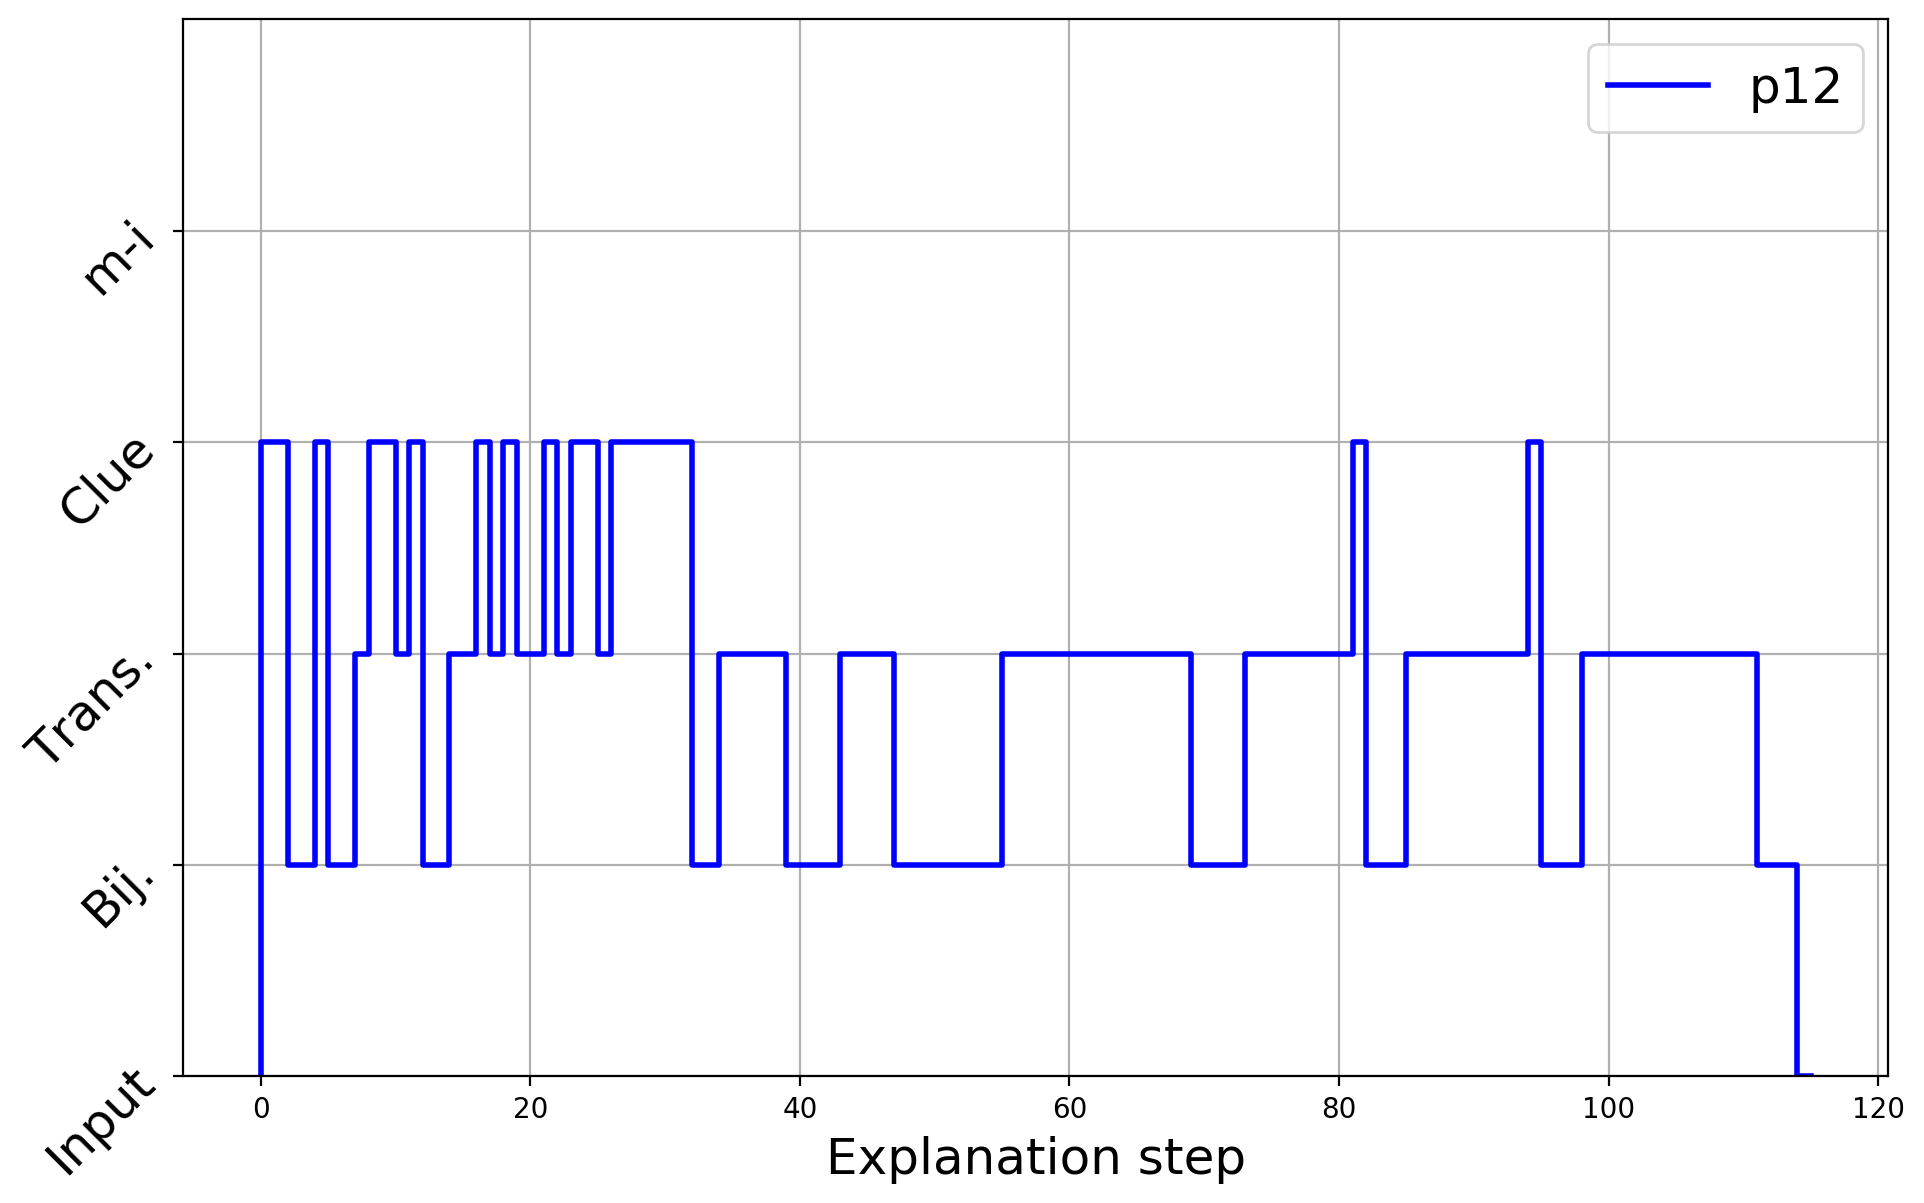
\includegraphics[width=0.49\linewidth]{figures/plot_cost_steps_p12}
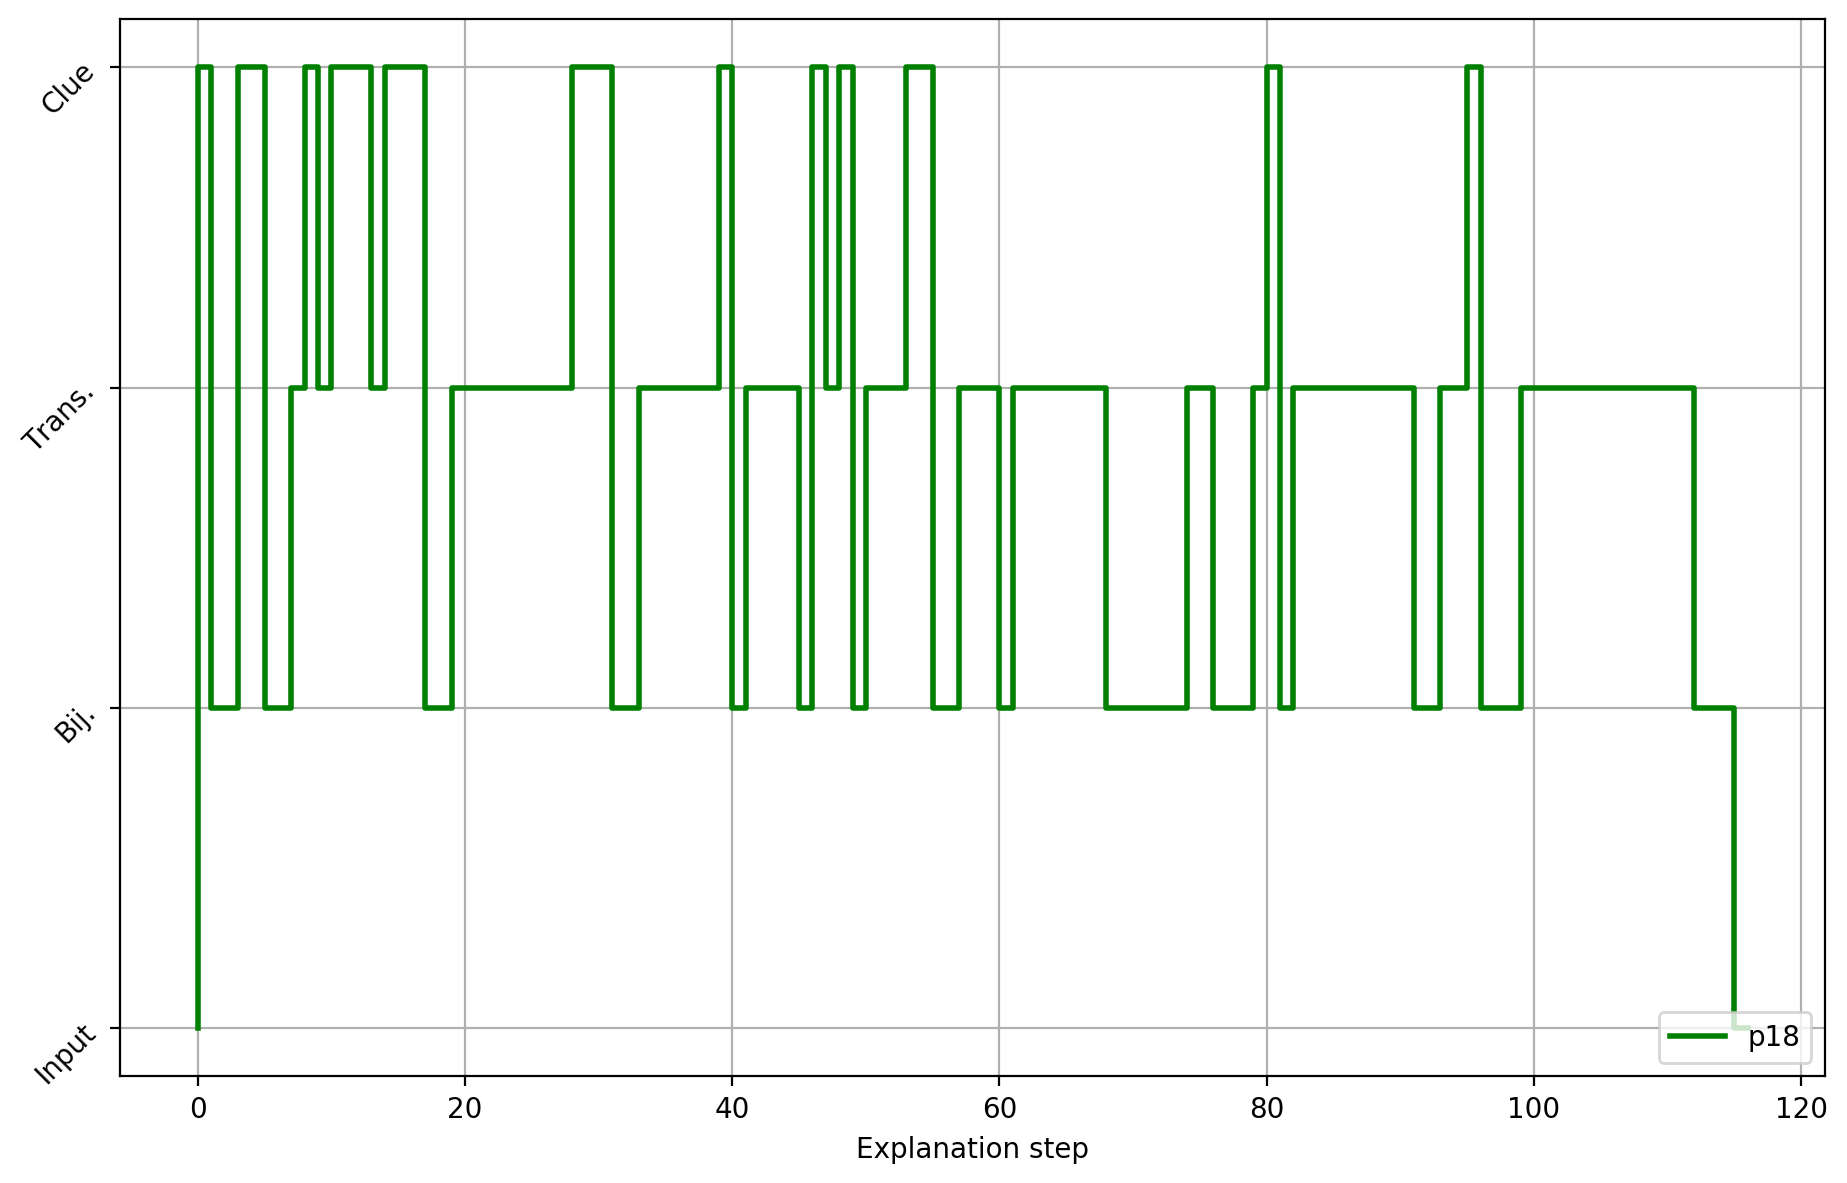
\includegraphics[width=0.49\linewidth]{figures/plot_cost_steps_p18}
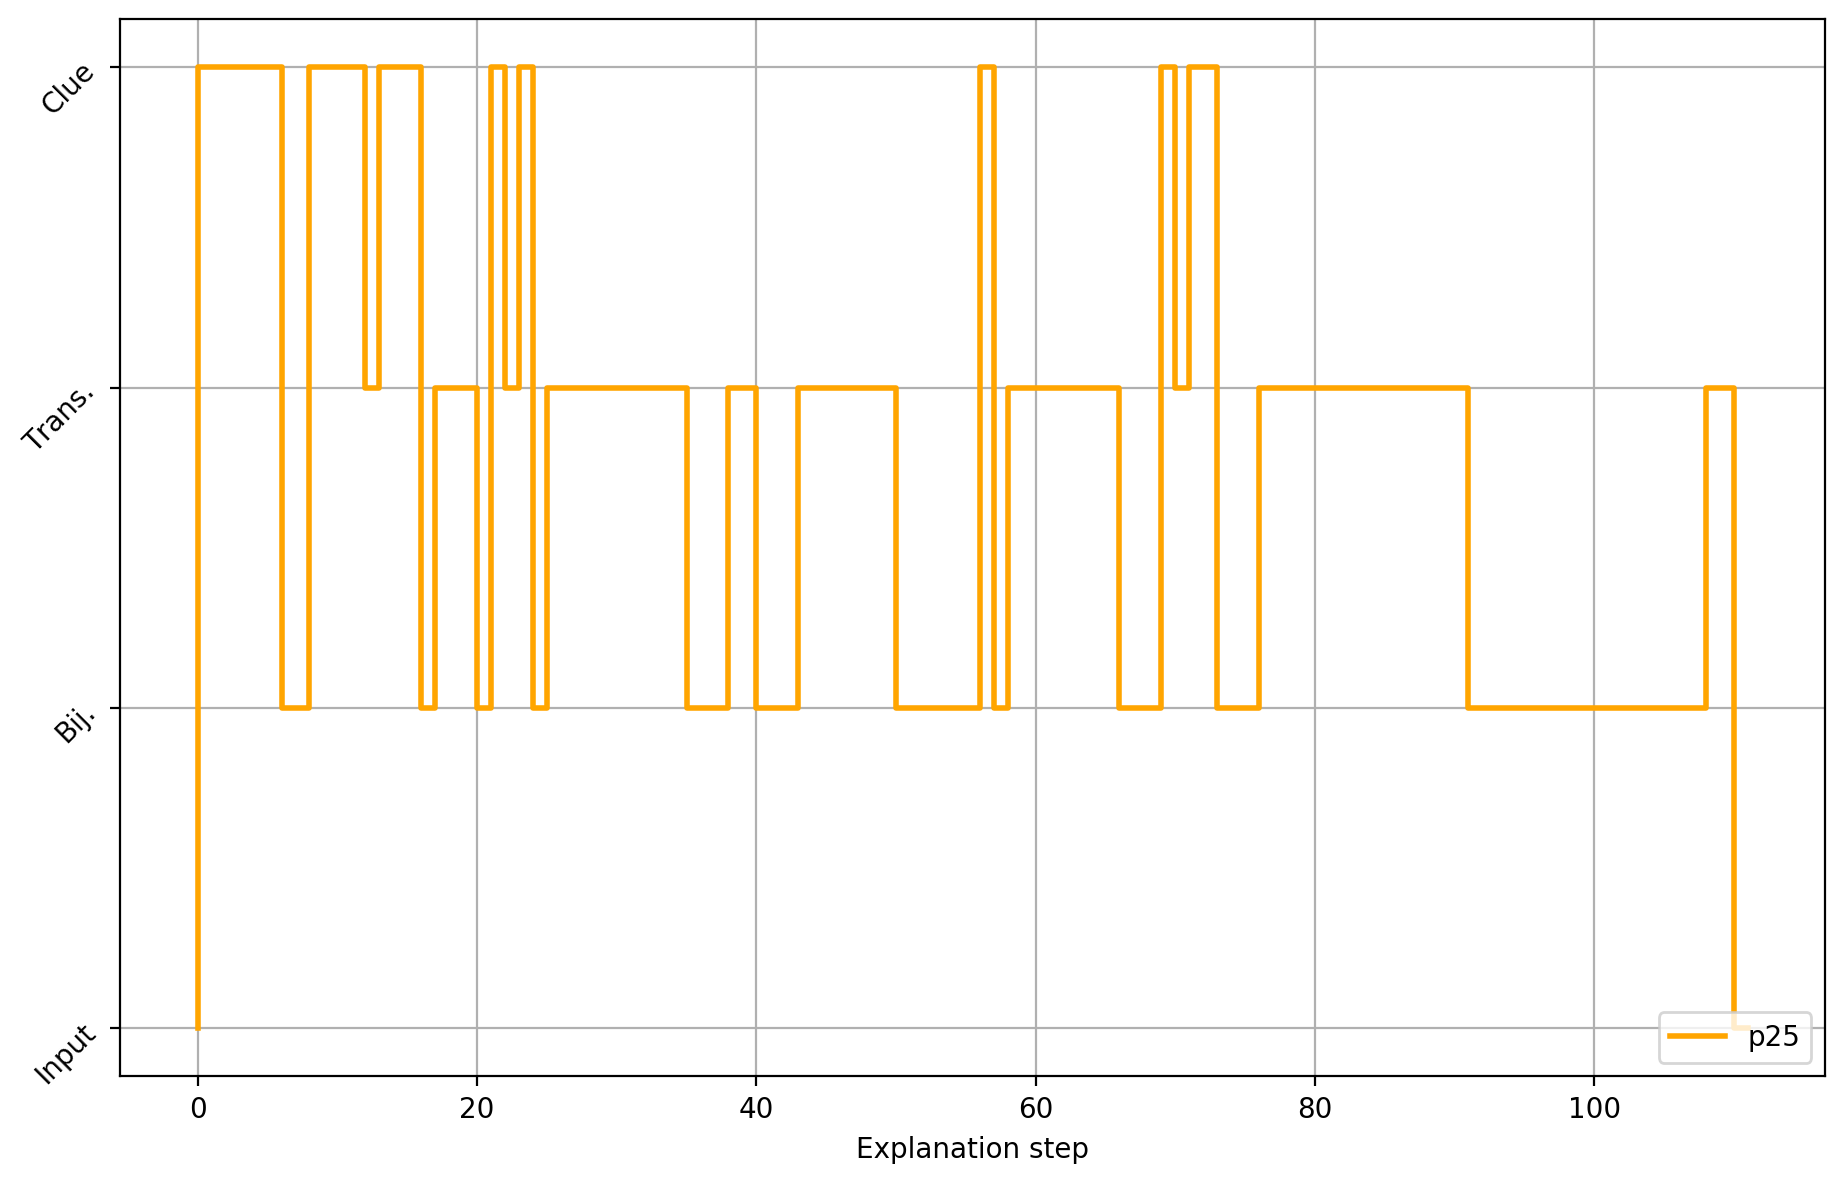
\includegraphics[width=0.49\linewidth]{figures/plot_cost_steps_p25}
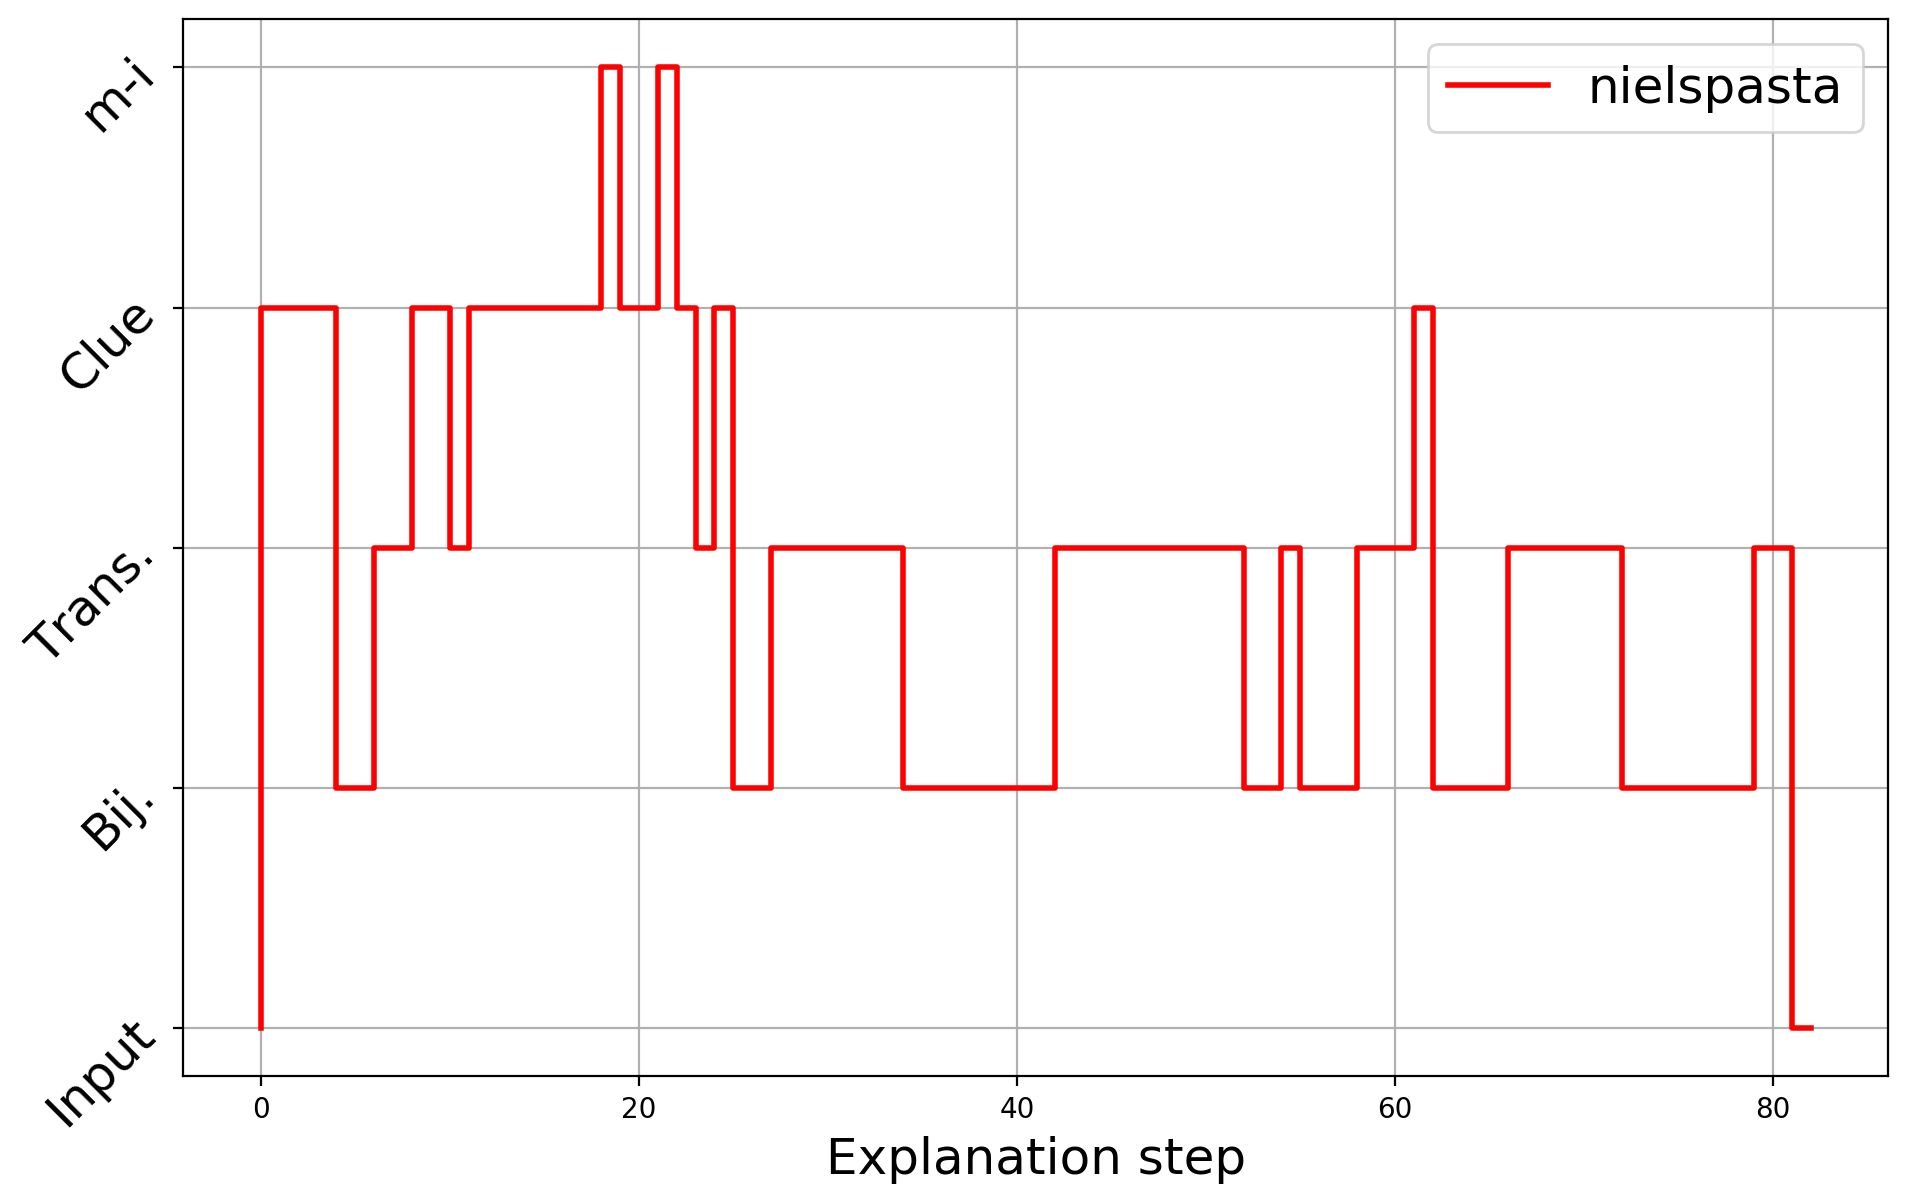
\includegraphics[width=0.49\linewidth]{figures/plot_cost_steps_nielspasta}
\caption{Type of constraints used in each step}
\label{fig:steps}
\end{figure}

\paragraph{3. Explanation size}
Our cost-function is constructed as to favor few (if any) clues and constraints in the explanations, and as few previously derived facts $|E|$. Table~\ref{table:sequence_leve} shows the average nr of facts use per explanation. We also show the average number of facts used when using only bijectivity or transitivity, or when a clue is used.

We can observe that the average number of facts used is indeed low, less than two. Further more, the breakdown shows that bijectivity typically uses more facts, e.g. it uses three 'negative' facts in one row to infer a 'positive' fact, as in Figure~\ref{fig:zebrascreen} or it uses one 'positive' fact to infer three negative facts. Note that for such an intuitive constraint, the number of facts used does not matter much. Transitivity, by nature, always uses two previously derived facts. Finally, when looking at the number of facts used together with a clue we can see that our approach succesfully finds small explanations: a number of clues (the trivial ones) use no facts, while most use 1 fact and rarely 2 facts are needed. \tias{Check when new table arrives}. The exception is again the difficult pasta puzzle, which \tias{check when new table arrives}.

\tias{Ideal table:}

\begin{table}
	\centering
	\resizebox{\columnwidth}{!}{%
		\begin{tabular}{l|c|ccc|cccc} 
		    & \multicolumn{4}{c|}{\bf avg. facts} & \multicolumn{4}{c}{\bf \% of clue expl. with facts} \\
			\textbf{p} & \textbf{all} & \textbf{Bij.} & \textbf{Trans.} & \textbf{Clues} & \textbf{0 facts} & \textbf{1 fact} & \textbf{2 facts} & \textbf{$>$2 facts}\\ 
			\hline 
			1 & 0 & 0 & 0 & 0 & 0 & 0 & 0 & 0 \\ 
		\end{tabular} 
	}
	\caption{Puzzle explanation cost based on the cost function $f(I, C)$ and statistics on puzzle constraints}
	\label{table:sequence_leve}
\end{table}

\begin{table}
	\centering
	\resizebox{\columnwidth}{!}{%
		\begin{tabular}{|l||c|c|c|c|} 
			\hline 
			\textbf{puzzle} & \textbf{avg. fact used} & \textbf{avg. facts used with a clue} & \textbf{avg. facts used with trans.} & \textbf{avg. facts used together with bij.}\\ 
			\hline 
			p5 & 1.823 & 0.524 & 2.371 & 2.0 \\ 
			\hline 
			p16 & 1.803 & 0.609 & 2.385 & 2.0 \\ 
			\hline 
			p93 & 1.84 & 0.182 & 2.575 & 2.0 \\ 
			\hline 
			p12 & 1.835 & 0.316 & 2.455 & 2.0 \\ 
			\hline 
			p18 & 1.853 & 0.45 & 2.5 & 2.0 \\ 
			\hline 
			p20 & 1.828 & 0.294 & 2.355 & 2.0 \\ 
			\hline 
			nielspasta & 1.768 & 1.05 & 2.071 & 2.0 \\ 
			\hline 
			p25 & 1.937 & 0.737 & 2.463 & 2.0 \\ 
			\hline 
			p19 & 1.87 & 0.4 & 2.6 & 2.0 \\ 
			\hline 
		\end{tabular} 
	}
	\caption{Puzzle explanation cost based on the cost function $f(I, C)$ and statistics on puzzle constraints}
	\label{table:sequence_leve}
\end{table}


%\paragraph{Bonus. How well does it compare to human solving process ?} 

% TODO Compare with the tutorial puzzle of logicgridpuzzles.com? Ideally, a small human evaluation (e.g. ask people to solve a 3-with-3 puzzle and note the order of derivations and clues used, compare this 'ranking' to our ranking, discuss some differences.

